% Options for packages loaded elsewhere
\PassOptionsToPackage{unicode}{hyperref}
\PassOptionsToPackage{hyphens}{url}
\PassOptionsToPackage{dvipsnames,svgnames*,x11names*}{xcolor}
%
\documentclass[
]{article}
\usepackage{lmodern}
\usepackage{amssymb,amsmath}
\usepackage{ifxetex,ifluatex}
\ifnum 0\ifxetex 1\fi\ifluatex 1\fi=0 % if pdftex
  \usepackage[T1]{fontenc}
  \usepackage[utf8]{inputenc}
  \usepackage{textcomp} % provide euro and other symbols
\else % if luatex or xetex
  \usepackage{unicode-math}
  \defaultfontfeatures{Scale=MatchLowercase}
  \defaultfontfeatures[\rmfamily]{Ligatures=TeX,Scale=1}
\fi
% Use upquote if available, for straight quotes in verbatim environments
\IfFileExists{upquote.sty}{\usepackage{upquote}}{}
\IfFileExists{microtype.sty}{% use microtype if available
  \usepackage[]{microtype}
  \UseMicrotypeSet[protrusion]{basicmath} % disable protrusion for tt fonts
}{}
\makeatletter
\@ifundefined{KOMAClassName}{% if non-KOMA class
  \IfFileExists{parskip.sty}{%
    \usepackage{parskip}
  }{% else
    \setlength{\parindent}{0pt}
    \setlength{\parskip}{6pt plus 2pt minus 1pt}}
}{% if KOMA class
  \KOMAoptions{parskip=half}}
\makeatother
\usepackage{xcolor}
\IfFileExists{xurl.sty}{\usepackage{xurl}}{} % add URL line breaks if available
\IfFileExists{bookmark.sty}{\usepackage{bookmark}}{\usepackage{hyperref}}
\hypersetup{
  colorlinks=true,
  linkcolor=blue,
  filecolor=Maroon,
  citecolor=Blue,
  urlcolor=Blue,
  pdfcreator={LaTeX via pandoc}}
\urlstyle{same} % disable monospaced font for URLs
\usepackage{longtable,booktabs}
% Correct order of tables after \paragraph or \subparagraph
\usepackage{etoolbox}
\makeatletter
\patchcmd\longtable{\par}{\if@noskipsec\mbox{}\fi\par}{}{}
\makeatother
% Allow footnotes in longtable head/foot
\IfFileExists{footnotehyper.sty}{\usepackage{footnotehyper}}{\usepackage{footnote}}
\makesavenoteenv{longtable}
\usepackage{graphicx}
\makeatletter
\def\maxwidth{\ifdim\Gin@nat@width>\linewidth\linewidth\else\Gin@nat@width\fi}
\def\maxheight{\ifdim\Gin@nat@height>\textheight\textheight\else\Gin@nat@height\fi}
\makeatother
% Scale images if necessary, so that they will not overflow the page
% margins by default, and it is still possible to overwrite the defaults
% using explicit options in \includegraphics[width, height, ...]{}
\setkeys{Gin}{width=\maxwidth,height=\maxheight,keepaspectratio}
% Set default figure placement to htbp
\makeatletter
\def\fps@figure{htbp}
\makeatother
\setlength{\emergencystretch}{3em} % prevent overfull lines
\providecommand{\tightlist}{%
  \setlength{\itemsep}{0pt}\setlength{\parskip}{0pt}}
\setcounter{secnumdepth}{5}


%% pandoc-tablenos: required package
\usepackage{caption}

%% pandoc-tablenos: environment to disable table caption prefixes
\makeatletter
\newcounter{tableno}
\newenvironment{tablenos:no-prefix-table-caption}{
  \caption@ifcompatibility{}{
    \let\oldthetable\thetable
    \let\oldtheHtable\theHtable
    \renewcommand{\thetable}{tableno:\thetableno}
    \renewcommand{\theHtable}{tableno:\thetableno}
    \stepcounter{tableno}
    \captionsetup{labelformat=empty}
  }
}{
  \caption@ifcompatibility{}{
    \captionsetup{labelformat=default}
    \let\thetable\oldthetable
    \let\theHtable\oldtheHtable
    \addtocounter{table}{-1}
  }
}
\makeatother

%% pandoc-secnos: required package
\usepackage{cleveref}

%% pandoc-eqnos: disable brackets around cleveref numbers
\creflabelformat{equation}{#2#1#3}
\ifluatex
  \usepackage{selnolig}  % disable illegal ligatures
\fi
\newlength{\cslhangindent}
\setlength{\cslhangindent}{1.5em}
\newlength{\csllabelwidth}
\setlength{\csllabelwidth}{3em}
\newenvironment{CSLReferences}[3] % #1 hanging-ident, #2 entry sp
 {% don't indent paragraphs
  \setlength{\parindent}{0pt}
  % turn on hanging indent if param 1 is 1
  \ifodd #1 \everypar{\setlength{\hangindent}{\cslhangindent}}\ignorespaces\fi
  % set line spacing
  % set entry spacing
  \ifnum #2 > 0
  \setlength{\parskip}{#3\baselineskip}
  \fi
 }%
 {}
\usepackage{calc} % for \widthof, \maxof
\newcommand{\CSLBlock}[1]{#1\hfill\break}
\newcommand{\CSLLeftMargin}[1]{\parbox[t]{\maxof{\widthof{#1}}{\csllabelwidth}}{#1}}
\newcommand{\CSLRightInline}[1]{\parbox[t]{\linewidth}{#1}}
\newcommand{\CSLIndent}[1]{\hspace{\cslhangindent}#1}

\author{}
\date{}

\begin{document}

\hypertarget{probability-and-bayes-theorem}{%
\section{Probability and Bayes
Theorem}\label{probability-and-bayes-theorem}}

\hypertarget{introduction}{%
\subsection{Introduction}\label{introduction}}

Probability theory is one of the three central mathematical tools in
machine learning, along with multivariable calculus and linear algebra.
Tools from probability allow us to manage the uncertainty inherent in
data collected from real world experiments, and to measure the
reliability of predictions that we might make from that data. In these
notes, we will review some of the basic terminology of probability and
introduce Bayesian inference as a technique in machine learning
problems.

This will only be a superficial introduction to ideas from probability.
For a thorough treatment, see
\href{https://probability.oer.math.uconn.edu/3160-oer}{this open-source
introduction to probability.} For a more applied emphasis, I recommend
the excellent online course
\href{https://ocw.mit.edu/courses/electrical-engineering-and-computer-science/6-041-probabilistic-systems-analysis-and-applied-probability-fall-2010/}{Probabilistic
Systems Analysis and Applied Probability} and its associated text
{[}\protect\hyperlink{ref-Bertsekas}{1}{]}.

\hypertarget{probability-basics}{%
\subsection{Probability Basics}\label{probability-basics}}

The theory of probability begins with a set \(X\) of possible events or
outcomes, together with a ``probability'' function \(P\) on (certain)
subsets of \(X\) that measures ``how likely'' that combination of events
is to occur.

The set \(X\) can be discrete or continuous. For example, when flipping
a coin, our set of possible events would be the discrete set \(\{H,T\}\)
corresponding to the possible events of flipping heads or tails. When
measuring the temperature using a thermometer, our set of possible
outcomes might be the set of real numbers, or perhaps an interval in
\(\mathbb{R}\). The thermometer's measurement is random because it is
affected by, say, electronic noise, and so its reading is the true
temperature perturbed by a random amount.

The values of \(P\) are between \(0\), meaning that the event \emph{will
not} happen, and \(1\), meaning that it is certain to occur. As part of
our set up, we assume that the total chance of some event from \(X\)
occurring is \(1\), so that \(P(X)=1\); and the chance of ``nothing''
happening is zero, so \(P(\emptyset)=0\). And if \(U\subset X\) is some
collection, then \(P(U)\) is the chance of an event from \(U\)
occurring.

The last ingredient of this picture of probability is additivity.
Namely, we assume that if \(U\) and \(V\) are subsets of \(X\) that are
disjoint, then \[
P(U\cup V)=P(U)+P(V).
\] Even more generally, we assume that this holds for (countably)
infinite collections of disjoint subsets \(U_1,U_2,\ldots\), where \[
P(U_1\cup U_2\cup\cdots)=\sum_{i=1}^{\infty} P(U_i)
\]

\textbf{Definition:} The combination of a set \(X\) of possible outcomes
and a probability function \(P\) on subsets of \(X\) that satisfies
\(P(X)=1\), \(0\le P(U)\le 1\) for all \(U\), and is additive on
countable disjoint collections of subsets of \(X\) is called a (naive)
probability space. \(X\) is called the \emph{sample space} and the
subsets of \(X\) are called \emph{events}.

\textbf{Warning:} The reason for the term ``naive'' in the above
definition is that, if \(X\) is an uncountable set such as the real
numbers \(\mathbb{R}\), then the conditions in the definition are
self-contradictory. This is a deep and rather surprising fact. To make a
sensible definition of a probability space, one has to restrict the
domain of the probability function \(P\) to certain subsets of \(X\).
These ideas form the basis of the mathematical subject known as measure
theory. In these notes we will work with explicit probability functions
and simple subsets such as intervals that avoid these technicalities.

\hypertarget{discrete-probability-examples}{%
\subsubsection{Discrete probability
examples}\label{discrete-probability-examples}}

The simplest probability space arises in the analysis of coin-flipping.
As mentioned earlier, the set \(X\) contains two elements \(\{H,T\}\).
The probability function \(P\) is determined by its value
\(P(\{H\})=p\), where \(0\le p\le 1\), which is the chance of the coin
yielding a ``head.'' Since \(P(X)=1\), we have \(P(\{T\})=1-p\).

Other examples of discrete probability spaces arise from dice-rolling
and playing cards. For example, suppose we roll two six-sided dice.
There are \(36\) possible outcomes from this experiment, each equally
likely. If instead we consider the sum of the two values on the dice,
our outcomes range from \(2\) to \(12\) and the probabilities of these
outcomes are given by

\begin{tablenos:no-prefix-table-caption}

\begin{longtable}[]{@{}llllllllllll@{}}
\toprule
2 & 3 & 4 & 5 & 6 & 7 & 8 & 9 & 10 & 11 & 12 &\tabularnewline
\midrule
\endhead
1/36 & 1/18 & 1/12 & 1/9 & 5/36 & 1/6 & 5/36 & 1/9 & 1/12 & 1/18 & 1/36
&\tabularnewline
\bottomrule
\end{longtable}

\end{tablenos:no-prefix-table-caption}

A traditional deck of \(52\) playing cards contains \(4\) aces. Assuming
that the chance of drawing any card is the same (and is therefore equal
to \(1/52\)), the probability of drawing an ace is \(4/52=1/13\) since
\[
P(\{A_{\clubsuit},A_{\spadesuit},A_{\heartsuit},A_{\diamondsuit}\}) = 4P(\{A_{\clubsuit}\})=4/52=1/13
\]

\hypertarget{continuous-probability-examples}{%
\subsubsection{Continuous probability
examples}\label{continuous-probability-examples}}

When the set \(X\) is continuous, such as in the temperature
measurement, we measure \(P(U)\), where \(U\subset X\), by giving a
``probability density function'' \(f:X\to \mathbb{R}\) and declaring
that \[
P(U) = \int_{U}f(x) dX.
\] Notice that our function \(f(x)\) has to satisfy the condition \[
P(X)=\int_{X} f(x)dX = 1.
\]

For example, in our temperature measurement example, suppose the
``true'' outside temperature is \(t_0\), and our thermometer gives a
reading \(t\). Then a good model for the random error is to assume that
the error \(x=t-t_0\) is governed by the density function \[
f_\sigma(x) = \frac{1}{\sigma\sqrt{2\pi}}e^{-x^2/2\sigma^2}
\] where \(\sigma\) is a parameter. In a continuous situation such as
this one, the probability of any particular outcome in \(X\) is zero
since \[
P(\{t\})=\int_{t}^{t}f_{\sigma}(x)dx = 0
\] Still, the shape of the density function does tell you where the
values are concentrated -- values where the density function is larger
are more likely than those where it is smaller.

With this density function, and x=\(t-t_0\), the error in our
measurement is given by \begin{equation}
P(|t-t_0|<\delta)=\int_{-\delta}^{\delta} \frac{1}{\sigma\sqrt{2\pi}}e^{-x^2/2\sigma^2} dx
\label{eq:normal}\end{equation}

The parameter \(\sigma\) (called the \emph{standard deviation}) controls
how tightly the thermometer's measurement is clustered around the true
value \(t_0\); when \(\sigma\) is large, the measurements are scattered
widely, when small, they are clustered tightly. See \cref{fig:density}.

\begin{figure}
\hypertarget{fig:density}{%
\centering
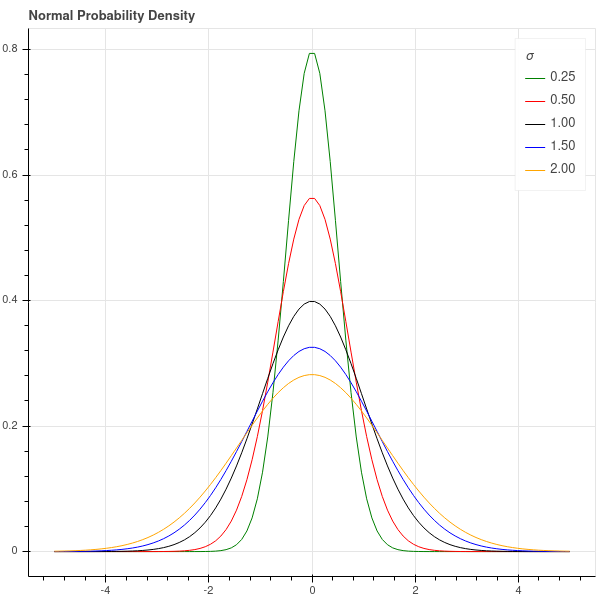
\includegraphics{../img/density.png}
\caption{Normal Density}\label{fig:density}
}
\end{figure}

\hypertarget{conditional-probability-and-bayes-theorem}{%
\subsection{Conditional Probability and Bayes
Theorem}\label{conditional-probability-and-bayes-theorem}}

The theory of conditional probability gives a way to study how partial
information about an event informs us about the event as a whole. For
example, suppose you draw a card at random from a deck. As we've seen
earlier, the chance that card is an ace is \(1/13\). Now suppose that
you learn that (somehow) that the card is definitely not a jack, king,
or queen. Since there are 12 cards in the deck that are jacks, kings, or
queens, the card you've drawn is one of the remaining 40 cards, which
includes 4 aces. Thus the chance you are holding an ace is now
\(4/40=1/10\).

In terms of notation, if \(A\) is the event ``my card is an ace'' and
\(B\) is the event ``my card is not a jack, queen, or king'' then we say
that \emph{the probability of \(A\) given \(B\)} is \(1/10\). The
notation for this is \[
P(A|B) = 1/10.
\]

More generally, if \(A\) and \(B\) are events from a sample space \(X\),
and \(P(B)>0\), then \[
P(A|B) = \frac{P(A\cap B)}{P(B)},
\] so that \(P(A|B)\) measures the chance that \(A\) occurs among those
situations in which \(B\) occurs.

\hypertarget{bayes-theorem}{%
\subsubsection{Bayes Theorem}\label{bayes-theorem}}

Bayes theorem is a foundational result in probability.

\textbf{Theorem:} Bayes Theorem says \[
P(A|B) = \frac{P(B|A)P(A)}{P(B)}.
\]

If we use the definition of conditional probability given above, this is
straightforward: \[
\frac{P(B|A)P(A)}{P(B)} = \frac{P(B\cap A)}{P(B)} = P(A|B).
\]

\hypertarget{an-example}{%
\subsubsection{An example}\label{an-example}}

To illustrate conditional probability, let's consider what happens when
we administer the most reliable COVID-19 test, the PCR test, to an
individual drawn from the population at large. There are two possible
test results (positive and negative) and two possible true states of the
person being tested (infected and not infected). Suppose I go to the
doctor and get a COVID test which comes back positive. What is the
probability that I actually have COVID?

Let's let \(S\) and \(W\) stand for infected (sick) and not infected
(well), and let \(+/-\) stand for test positive or negative. Note that
there are four possible outcomes of our experiment:

\begin{itemize}
\tightlist
\item
  test positive and infected (S+) -- this is a \emph{true positive}.
\item
  test positive and not infected (W+) -- this is a \emph{false
  positive}.
\item
  test negative and infected (S-) -- this is a \emph{false negative}.
\item
  test negative and not infected (W-) -- this is a \emph{true negative}.
\end{itemize}

The
\href{https://www.icd10monitor.com/false-positives-in-pcr-tests-for-covid-19}{CDC
says} that the chance of a false positive -- that is, the percentage of
samples from well people that incorrectly yields a positive result -- is
about one-half of one percent, or 5 in 1000.

In other words, \[
P(+|W) = P(W+)/P(W) = 5/1000=1/200
\]

On the other hand, the CDC tells us that chance of a false negative is 1
in 4, so \[
P(-|S) = P(S-)/P(S) = .25.
\] Since \(P(S-)+P(S+)=P(S).\) since every test is either positive or
negative, we have \[
P(+|S) = .75.
\]

Suppose furthermore that the overall incidence of COVID-19 in the
population is p.~In other words, \(P(S)=p\) so \(P(W)=1-p\). Then
\[P(S+)=P(S)P(+|S)=.75p\] and \[
P(W+)=P(W)P(+|W)=.005(1-p).
\] Putting these together we get \(P(+)=.005+.745p\)

What I'm interested in is \(P(S|+)\) -- the chance that I'm sick, given
that my test result was positive. By Bayes Theorem, \[
P(S|+)=\frac{P(+|S)P(S)}{P(+)}=.75p/(.005+.745p)=\frac{750p}{5+745p}.
\]

As \cref{fig:covidfn} shows, if the population incidence is low then a
positive test is far from conclusive. Indeed, if the overall incidence
of COVID is one percent, then a positive test result only implies a 60
percent chance that I am in fact infected.

Just to fill out the picture, we have \[
P(-) = P(S-)+P(W-)=(P(S)-P(S+))+(P(W)-P(W+))
\] which yields \[
P(-)=1-.005+.005p-.75p = .995-.745p.
\] Using Bayes Theorem, we obtain \[
P(S|-) = \frac{P(-|S)P(S)}{P(-)} = .25p/(.995-.745p) =\frac{250p}{995-745p}.
\] In this case, even though the false negative rate is pretty high (25
percent) overall, if the population incidence is one percent, then the
probability that you're sick given a negative result is only about
\(.25\) percent. So negative results are very likely correct!

\begin{figure}
\hypertarget{fig:covidfn}{%
\centering
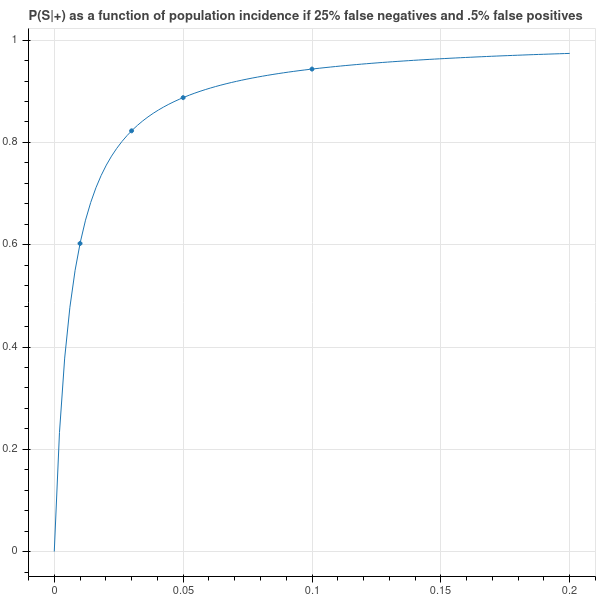
\includegraphics{../img/covidfn.png}
\caption{P(S\textbar+) vs P(S)}\label{fig:covidfn}
}
\end{figure}

\hypertarget{independence}{%
\subsection{Independence}\label{independence}}

Independence is one of the fundamental concepts in probability theory.
Conceptually, two events are independent if the occurrence of one has
does not influence the likelihood of the occurrence of the other. For
example, successive flips of a coin are independent events, since the
result of the second flip doesn't have anything to do with the result of
the first. On the other hand, whether or not it rains today and tomorrow
are not independent events, since the weather tomorrow depends (in a
complicated way) on the weather today.

We can formalize this idea of independence using the following
definition.

\textbf{Definition:} Let \(X\) be a sample space and let \(A\) and \(B\)
be two events. Then \(A\) and \(B\) are \emph{independent} if
\(P(A\cap B)=P(A)P(B)\). Equivalently, \(A\) and \(B\) are independent
if \(P(A|B)=P(A)\) and \(P(B|A)=P(B)\).

\hypertarget{examples}{%
\subsubsection{Examples}\label{examples}}

\hypertarget{coin-flipping}{%
\paragraph{Coin Flipping}\label{coin-flipping}}

Suppose our coin has a probability of heads given by a real number \(p\)
between \(0\) and \(1\), and we flip our coin \(N\) times. What is the
chance of gettting \(k\) heads, where \(0\le k\le N\)? Any particular
sequence of heads and tails containing \(k\) heads and \(N-k\) tails has
probability \[
P(\hbox{\rm particular sequence of $k$ heads among $N$ flips}) = p^{k}(1-p)^{N-k}.
\] In addition, there are \(\binom{N}{k}\) sequences of heads and tails
containing \(k\) heads. Thus the probability \(P(k,N)\) of \(k\) heads
among \(N\) flips is \begin{equation}
P(k,N) = \binom{N}{k}p^{k}(1-p)^{N-k}.
\label{eq:binomial}\end{equation}

Notice that the binomial theorem gives us \(\sum_{k=0}^{N} P(k,N) =1\)
which is a reassuring check on our work.

The probability distribution on the set \(X=\{0,1,\ldots,N\}\) given by
\(P(k,N)\) is called the \emph{binomial distribution} with parameters
\(N\) and \(p\).

\hypertarget{a-simple-mixture}{%
\paragraph{A simple `mixture'}\label{a-simple-mixture}}

Now let's look at an example of events that are not independent. Suppose
that we have two coins, with probabilities of heads \(p_1\) and \(p_2\)
respectively; and assume these probabilities are different. We play the
a game in which we first choose one of the two coins (with equal chance)
and then flip it twice. Is the result of the second flip independent of
the first? In other words, is \(P(HH)=P(H)^2\)?

This type of situation is called a `mixture distribution' because the
probability of a head is a ``mixture'' of the probability coming from
the two different coins.

The chance that the first flip is a head is \((p_1+p_2)/2\) because it's
the chance of picking the first coin, and then getting a head, plus the
chance of picking the second, and then getting a head. The chance of
getting two heads in a row is \((p_1^2+p_2^2)/2\) because it's the
chance, having picked the first coin, of getting two heads, plus the
chance, having picked the second, of getting two heads.

Since \[
\frac{p_1^2+p_2^2}{2}\not=\left(\frac{p_1+p_2}{2}\right)^2
\] we see these events are not independent.

In terms of conditional probabilities, the chance that the second flip
is a head, given that the first flip is, is computed as: \[
P(HH|H) = \frac{p_1^2+p_2^2}{p_1+p_2}.
\] From the Cauchy-Schwartz inequality one can show that \[
\frac{p_1^2+p_2^2}{p_1+p_2}>\frac{p_1+p_2}{2}.
\]

Why should this be? Why should the chance of getting a head on the
second flip go up given that the first flip was a head? One way to think
of this is that the first coin flip contains a little bit of information
about which coin we chose. If, for example \(p_1>p_2\), and our first
flip is heads, then it's just a bit more likely that we chose the first
coin. As a result, the chance of getting another head is just a bit more
likely than if we didn't have that information. We can make this precise
by considering the conditional probability \(P(p=p_1|H)\) that we've
chosen the first coin given that we flipped a head. From Bayes' theorem:

\[
P(p=p_1|H) = \frac{P(H|p=p_1)P(p=p_1)}{P(H)}=\frac{p_1}{p_1+p_2}=\frac{1}{1+(p_2/p_1)}>\frac{1}{2}
\] since \((1+(p_2/p_1))<2\).

\textbf{Exercise:} Push this argument a bit further. Let
\(p_1=\max(p_1,p_2)\) Let \(P_N\) be the conditional probability of
getting heads assuming that the first \(N\) flips were heads. Show that
\(P_N\to p_1\) as \(N\to\infty\). All those heads piling up make it more
and more likely that you're flipping the first coin and so the chance of
getting heads approaches \(p_1\).

\hypertarget{an-example-with-a-continuous-distribution}{%
\paragraph{An example with a continuous
distribution}\label{an-example-with-a-continuous-distribution}}

Suppose that we return to our example of a thermometer which measures
the ambient temperature with an error that is distributed according to
the normal distribution, as in \cref{eq:normal}. Suppose that we make 10
independent measurements \(t_1,\ldots, t_{10}\) of the true temperature
\(t_0\). What can we say about the distribution of these measurements?

In this case, independence means that \[
P=P(|t_1-t_0|<\delta,|t_2-t_0|<\delta,\ldots) = P(|t_1-t_0|<\delta)P(|t_2-t_0|<\delta)\cdots P(|t_{10}-t_{0}|<\delta)
\] and therefore \[
P = \left(\frac{1}{\sigma\sqrt{2\pi}}\right)^{10}\int_{-\delta}^{\delta}\cdots\int_{-\delta}^{\delta}
e^{-(\sum_{i=1}^{10} x_i^2)/2\sigma^2} dx_1\cdots dx_{10}
\]

One way to look at this is that the vector \(\mathbf{e}\) of errors
\((|t_1-t_0|,\ldots,|t_{10}-t_0|)\) is distributed according to a
\emph{multivariate gaussian distribution}: \begin{equation}
P(\mathbf{e}\in U) =\left(\frac{1}{\sigma\sqrt{2\pi}}\right)^{10}\int_{U} 
e^{-\|x\|^2/2\sigma^2} d\mathbf{x}
\label{eq:multivariategaussian}\end{equation}

where \(U\) is a region in \(\mathbf{R}^{10}\).

The multivariate gaussian can also describe situations where
independence does not hold. For simplicity, let's work in two dimensions
and consider the probability density on \(\mathbf{R}^{2}\) given by \[
P(\mathbf{e}\in U) = A\int_{U} e^{-(x_1^2-x_1x_2+x_2^2)/2\sigma^2} d\mathbf{x}.
\] where the constant \(A\) is chosen so that \[
A\int_{\mathbf{R}^{2}}e^{-(x_1^2-x_1x_2+x_2^2)/2\sigma^2}d\mathbf{x} = 1.
\]

This density function as a ``bump'' concentrated near the origin in
\(\mathbf{R}^{2}\), and its level curves are a family of ellipses
centered at the origin. See \cref{fig:multivariate} for a plot of this
function with \(\sigma=1\).

\begin{figure}
\hypertarget{fig:multivariate}{%
\centering
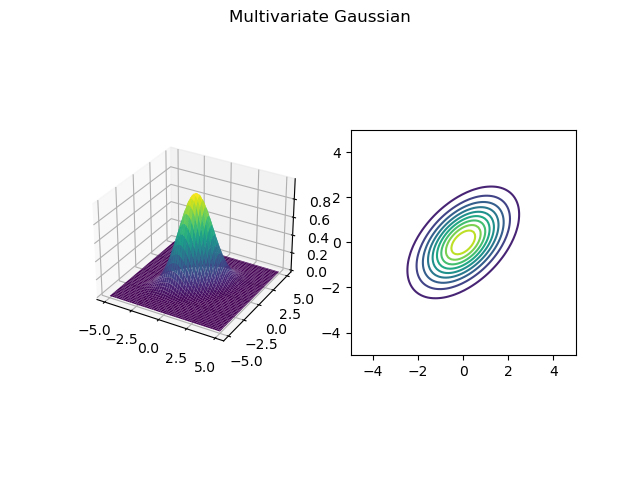
\includegraphics{../img/ellipse.png}
\caption{Multivariate Gaussian}\label{fig:multivariate}
}
\end{figure}

In this situation we can look at the conditional probability of the
first variable given the second, and see that the two variables are not
independent. Indeed, if we fix \(x_2\), then the distribution of \(x_1\)
depends on our choice of \(x_2\). We could see this by a calculation, or
we can just look at the graph: if \(x_2=0\), then the most likely values
of \(x_1\) cluster near zero, while if \(x_2=1\), then the most likely
values of \(x_1\) cluster somewhere above zero.

\hypertarget{random-variables-mean-and-variance}{%
\subsection{Random Variables, Mean, and
Variance}\label{random-variables-mean-and-variance}}

Typically, when we are studying a random process, we aren't necessarily
accessing the underlying events, but rather we are making measurements
that provide us with some information about the underlying events. For
example, suppose our sample space \(X\) is the set of throws of a pair
of dice, so \(X\) contains the \(36\) possible combinations that can
arise from the throws. What we are actually interested is the sum of the
values of the two dice -- that's our ``measurement'' of this system.
This rather vague notion of a measurement of a random system is captured
by the very general idea of a \emph{random variable}.

\textbf{Definition:} Let \(X\) be a sample space with probability
function \(P\). A \emph{random variable} on \(X\) is a function
\(f:X\to \mathbb{R}\).

Given a random variable \(f\), we can use the probability measure to
decide how likely \(f\) is to take a particular value, or values in a
particular set by the formula \[
P(f(x)\in U) = P(f^{-1}(U))
\]

In the dice rolling example, the random variable \(S\) that assigns
their sum to the pair of values obtained on two dice is a random
variable. Those values lie between \(2\) and \(12\) and we have \[
P(S=k) = P(S^{-1}(\{k\}))=P(\{(x,y): x+y=k\})
\] where \((x,y)\) runs through \(\{1,2,\ldots,6\}^{2}\) representing
the two values and \(P((x,y))=1/36\) since all throws are equally
likely.

Let's look at a few more examples, starting with what is probably the
most fundamental of all.

\textbf{Definition:} Let \(X\) be a sample space with two elements, say
\(H\) and \(T\), and suppose that \(P(H)=p\) for some \(0\le p\le 1\).
Then the random variable that satisfies \(f(H)=1\) and \(f(T)=0\) is
called a Bernoulli random variable with parameter \(p\).

In other words, a Bernoulli random variable gives the value \(1\) when a
coin flip is heads, and \(0\) for tails.

Now let's look at what we earlier called the binomial distribution.

\textbf{Definition:} Let \(X\) be a sample space consisting of strings
of \(H\) and \(T\) of length \(N\), with the probability of a
\emph{particular string} \(S\) with \(k\) heads and \(N-k\) tails given
by \[
P(S)=p^{k}(1-p)^{N-k}
\] for some \(0\le p\le 1\). In other words, \(X\) is the sample space
consisting of \(N\) independent flips of a coin with probability of
heads given by \(p\).\\
Let \(f:X\to \mathbb{R}\) be the function which counts the number of
\(H\) in the string. Then \(f\) is a random variable called a
\emph{binomial random variable} with parameters \(p\) and \(N\).
Clearly, a binomial random variable with \(N=1\) is just a Bernoulli
variable with parameter \(p\).

If \(f\) is a binomial random variable with parameters \(p\) and \(N\),
then \[
P(f=k) = \binom{N}{k}p^{k}(1-p)^{N-k}
\] since \(f^{-1}(\{k\})\) is the number of elements in the subset of
strings of \(H\) and \(T\) of length \(N\) containing exactly \(k\)
\(H\)'s.

For an example with a continuous random variable, suppose our sample
space is \(\mathbf{R}^{2}\) and the probability density is the simple
multivariate normal \[
P(\mathbf{x}\in U) = \left(\frac{1}{\sqrt{2\pi}}\right)^2\int_{U} e^{-\|\mathbf{x}\|^2/2} d\mathbf{x}.
\] Let \(f\) be the random variable \(f(\mathbf{x})=\|\mathbf{x}\|\).
The function \(f\) measures the Euclidean distance of a randomly drawn
point from the origin. The set
\[U=f^{-1}([0,r))\subseteq\mathbf{R}^{2}\] is the circle of radius \(r\)
in \(\mathbf{R}^{2}\). The probability that a randomly drawn point lies
in this circle is \[
P(f<r) = \left(\frac{1}{\sqrt{2\pi}}\right)^2\int_{U} e^{-\|\mathbf{x}\|^2/2} d\mathbf{x}.
\]

We can actually evaluate this integral in closed form by using polar
coordinates. We obtain \[
P(f<r) = \left(\frac{1}{\sqrt{2\pi}}\right)^2\int_{\theta=0}^{2\pi}\int_{\rho=0}^{r} e^{-\rho^2/2}\rho d\rho d\theta.
\] Since \[
\frac{d}{d\rho}e^{-\rho^2/2}=-\rho e^{-\rho^2/2}
\] we have \begin{align*}
P(f<r)&=-\frac{1}{2\pi}\theta e^{-\rho^2/2}|_{\theta=0}^{2\pi}|_{\rho=0}^{r}\cr
&=1-e^{-r^2/2}\cr
\end{align*}

The probability density associated with this random variable is the
derivative of \(1-e^{-r^2/2}\) \[
P(f\in [a,b])=\int_{r=a}^{b} re^{-r^2/2} dr
\] as you can see by the fundamental theorem of calculus. This density
is drawn in \cref{fig:maxwell} where you can see that the points are
clustered at a distance of \(1\) from the origin.

\begin{figure}
\hypertarget{fig:maxwell}{%
\centering
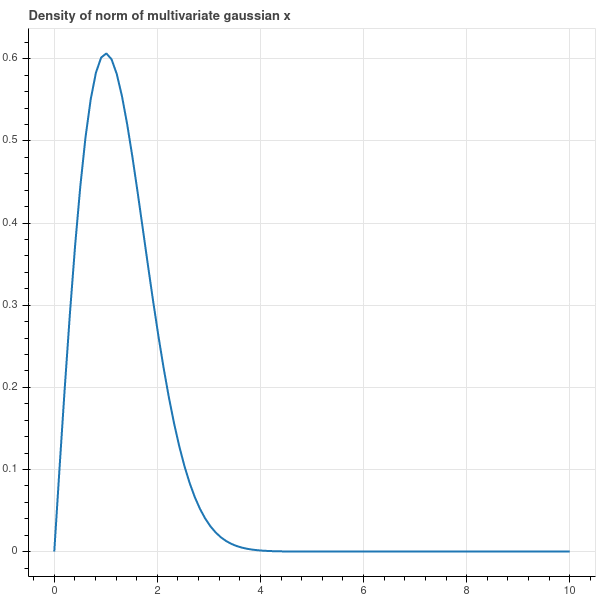
\includegraphics{../img/maxwell.png}
\caption{Density of the Norm}\label{fig:maxwell}
}
\end{figure}

\hypertarget{independence-and-random-variables}{%
\subsubsection{Independence and Random
Variables}\label{independence-and-random-variables}}

We can extend the notion of independence from events to random
variables.

\textbf{Definition:} Let \(f\) and \(g\) be two random variables on a
sample space \(X\) with probability \(P\). Then \(f\) and \(g\) are
independent if, for all intervals \(U\) and \(V\) in \(\mathbb{R}\), the
events \(f^{-1}(U)\) and \(g^{-1}(V)\) are independent.

For discrete probability distributions, this means that, for all
\(a,b\in\mathbb{R}\), \[
P(f=a\hbox{\rm\ and\ }g=b)=P(f=a)P(g=b).
\]

For continous probability distributions given by a density function
\(P(x)\), independence can be more complicated to figure out.

\hypertarget{expectation-mean-and-variance}{%
\subsubsection{Expectation, Mean and
Variance}\label{expectation-mean-and-variance}}

The most fundamental tool in the study of random variables is the
concept of ``expectation,'' which is a fancy version of average. The
word ``mean'' is a synonym for expectation -- the mean of a random
variable is the same as its expectation or ``expected value.''

\textbf{Definition:} Let \(X\) be a sample space with probability
measure \(P\). Let \(f:X\to \mathbb{R}\) be a random variable. Then the
\emph{expectation} or \emph{expected value} \(E[f]\) of \(f\) is \[
E[f] = \int_X f(x)dP.
\] More specifically, if \(X\) is discrete, then \[
E[f] = \sum_{x\in X} f(x)P(x)
\] while if \(X\) is continuous with probability density function
\(p(x)dx\) then \[
E[f] = \int_{X} f(x)p(x)dx.
\]

If \(f\) is a Bernoulli random variable with parameter \(p\), then \[
E[f] = 1\cdot p+0\cdot (1-p) = p
\]

If \(f\) is a binomial random variable with parameters \(p\) and \(N\),
then \[
E[f] = \sum_{i=0}^{N} i\binom{N}{i}p^{i}(1-p)^{N-i}
\] One can evaluate this using some combinatorial tricks, but it's
easier to apply this basic fact about expectations.

\textbf{Proposition:} Expectation is linear: \(E[aX+bY]=aE[X]+bE[Y]\)
for random variables \(X,Y\) and constants \(a\) and \(b\).

The proof is an easy consequence of the expression of \(E\) as a sum (or
integral).

Since a binomial random variable \(Z\) with parameters \(N\) and \(p\)
is the sum of \(N\) Bernoulli random variables, its expectation is \[
E[X_1+\cdots+X_N]=Np.
\]

A more sophisticated property of expectation is that it is
multiplicative when the random variables are independent.

\textbf{Proposition:} Let \(f\) and \(g\) be two independent random
variables. Then \(E[fg]=E[f]E[g]\).

\textbf{Proof:} Let's suppose that the sample space \(X\) is discrete.
By definition, \[
E[f]=\sum_{x\in X}f(x)P(x)
\] and we can rewrite this as \[
E[f]=\sum_{a\in\mathbf{R}} aP(\{x: f(x)=a\}).
\] Let \(Z\subset\mathbb{R}\) be the range of \(f\). Then \begin{align*}
E[fg]&=\sum_{a\in Z} aP(\{x: fg(x)=a\}) \\
&=\sum_{a\in Z}\sum_{(u,v)\in\genfrac{}{}{0pt}{}{\mathbf{Z}^{2}}{uv=a}}aP(\{x:f(x)=u\hbox{\rm\ and\ }g(x)=v\}) \\
&=\sum_{a\in Z}\sum_{\genfrac{}{}{0pt}{}{\mathbf{Z}^{2}}{uv=a}}uvP(\{x:f(x)=u\})P(\{x:g(x)=v\}) \\
&=\sum_{u\in Z}uP(\{x:f(x)=u\})\sum_{v\in Z}vP(\{x:f(x)=v\}) \\
&=E[f]E[g] 
\end{align*}

\hypertarget{variance}{%
\paragraph{Variance}\label{variance}}

The variance of a random variable is a measure of its dispersion around
its mean.

\textbf{Definition:} Let \(f\) be a random variable. Then the variance
is the expression \[
\sigma^2(f) = E[(f-E[f])^2]=E[f^2]-(E[f])^2
\] The square root of the variance is called the ``standard deviation.''

The two formulae for the variance arise from the calculation \[
E[(f-E[f])^2]=E[(f^2-2fE[f]+E[f]^2)]=E[f^2]-2E[f]^2+E[f]^2=E[f^2]-E[f]^2.
\]

To compute the variance of the Bernoulli random variable \(f\) with
parameter \(p\), we first compute \[
E[f^2]=p(1)^2+(1-p)0^2=p.
\] Since \(E[f]=p\), we have \[
\sigma^2(f)=p-p^2=p(1-p).
\]

If \(f\) is the binomial random variable with parameters \(N\) and
\(p\), we can again use the fact that \(f\) is the sum of \(N\)
Bernoulli random variables \(X_1+\cdots+X_n\) and compute

\begin{align*}
E[(\sum_{i}X_i)^2]-E[\sum_{i} X_{i}]^2 &=E[\sum_{i} X_i^2+\sum_{i,j}X_{i}X_{j}]-N^2p^2\\
&=Np+N(N-1)p^2-N^2p^2 \\
&=Np(1-p)
\end{align*}

where we have used the fact that the square \(X^2\) of a Bernoulli
random variable is equal to \(X\).

For a continuous example, suppose that we consider a sample space
\(\mathbb{R}\) with the normal probability density \[
P(x) = \frac{1}{\sigma\sqrt{2\pi}}e^{-x^2/2\sigma^2}dx.
\]

The mean of the random variable \(x\) is \[
E[x] =\frac{1}{\sigma\sqrt{2\pi}}\int_{-\infty}^{\infty} xe^{-x^2/2\sigma^2}dx=0
\]

since the function being integrated is odd. The variance is

\[
E[x^2] = \frac{1}{\sigma\sqrt{2\pi}}\int_{-\infty}^{\infty} x^2e^{-x^2/2\sigma^2}dx.
\]

The trick to evaluating this integral is to consider the derivative:

\[
\frac{d}{d\sigma}\left[\frac{1}{\sigma\sqrt{2\pi}}\int_{-\infty}^{\infty}e^{-x^2/(2\sigma^2)}dx\right]=0
\]

where the result is zero since the quantity being differentiated is a
constant (namely \(1\)). Sorting through the resulting equation leads to
the fact that

\[
E[x^2]=\sigma^2
\]

so that the \(\sigma^2\) parameter in the normal distribution really
\emph{is} the variance of the associated random variable.

\hypertarget{models-and-likelihood}{%
\subsection{Models and Likelihood}\label{models-and-likelihood}}

A \emph{statistical model} is a mathematical model that accounts for
data via a process that incorporates random behavior in a structured
way. We have seen several examples of such models in our discussion so
far. For example, the Bernoulli process that describes the outcome of a
series of coin flips as independent choices of heads or tails with
probability \(p\) is a simple statistical model; our more complicated
mixture model in which we choose one of two coins at random and then
flip that is a more complicated model.\\
Our description of the variation in temperature measurements as arising
from perturbations from the true temperature by a normally distributed
amount is another example of a statistical model, this one involving a
continuous random variable.

When we apply a mathematical model to understand data, we often have a
variety of parameters in the model that we must adjust to get the model
to best ``fit'' the observed data. For example, suppose that we observe
the vibrations of a block attached to a spring. We know that the motion
is governed by a second order linear differential equation, but the
dynamics depend on the mass of the block, the spring constant, and the
damping coefficient. By measuring the dynamics of the block over time,
we can try to work backwards to figure out these parameters, after which
we will be able to predict the block's motion into the future.

\hypertarget{sec:mlcoin}{%
\subsubsection{Maximum Likelihood (Discrete Case)}\label{sec:mlcoin}}

To see this process in a statistical setting, let's return to the simple
example of a coin flip. The only parameter in our model is the
probability \(p\) of getting heads on a particular flip. Suppose that we
flip the coin \(100\) times and get \(55\) heads and \(45\) tails. What
can we say about \(p\)?

We will approach this question via the ``likelihood'' function for our
data. We ask: for a particular value of the parameter \(p\), how likely
is this outcome? From \cref{eq:binomial} we have \[
P(55H,45T)=\binom{100}{55}p^{55}(1-p)^{45}.
\]

This function is plotted in \cref{fig:beta}. As you can see from that
plot, it is extremely unlikely that we would have gotten \(55\) heads if
\(p\) was smaller than \(.4\) or greater than \(.7\), while the
\emph{most likely} value of \(p\) occurs at the maximum value of this
function, and a little calculus tells us that this point is where
\(p=.55\). This \emph{most likely} value of \(p\) is called the
\emph{maximum likelihood estimate} for the parameter \(p\).

\begin{figure}
\hypertarget{fig:beta}{%
\centering
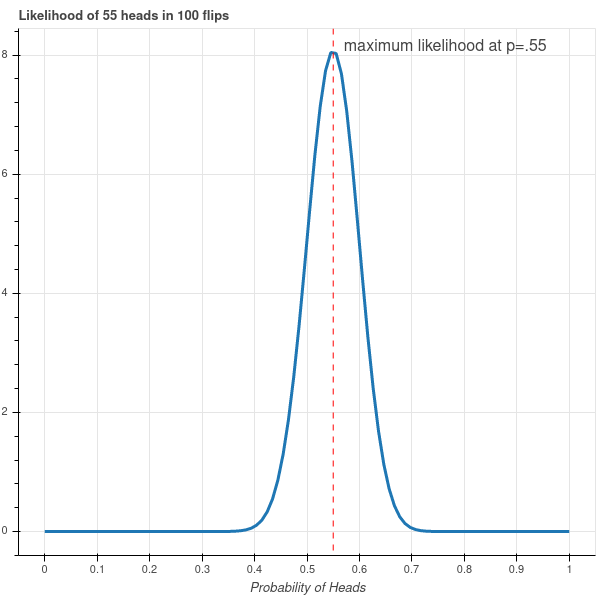
\includegraphics{../img/beta.png}
\caption{Likelihood Plot}\label{fig:beta}
}
\end{figure}

\hypertarget{maximum-likelihood-continuous-case}{%
\subsubsection{Maximum Likelihood (Continuous
Case)}\label{maximum-likelihood-continuous-case}}

Now let's look at our temperature measurements where the error is
normally distributed with variance parameter \(\sigma^2\). As we have
seen earlier, the probability density of errors
\(\mathbf{x}=(x_1,\ldots,x_n)\) of \(n\) independent measurements is \[
P(\mathbf{x}) = \left(\frac{1}{\sigma\sqrt{2\pi}}\right)^{n}e^{-\|\mathbf{x}\|^2/(2\sigma^2)}d\mathbf{x}.
\] (see \cref{eq:multivariategaussian}). What should we use as the
parameter \(\sigma\)? We can ask which choice of \(\sigma\) makes our
data \emph{most likely}. To calculate this, we think of the probability
of a function of \(\sigma\) and use Calculus to find the maximum. It's
easier to do this with the logarithm.

\[
\log P(\mathbf{x})=\frac{-\|\mathbf{x}\|^2}{2\sigma^2}-n\log{\sigma}+C
\] where \(C\) is a constant that we'll ignore. Taking the derivative
and setting it to zero, we obtain \[
-\|\mathbf{x}\|^2\sigma^{-3}-n\sigma^{-1}=0
\] which gives the formula \[
\sigma^2=\frac{\|\mathbf{x}\|^2}{n}
\]

This should look familiar! The maximum likelihood estimate of the
variance is the \emph{mean-squared-error}.

\hypertarget{linear-regression-and-likelihood}{%
\subsubsection{Linear Regression and
likelihood}\label{linear-regression-and-likelihood}}

In our earlier lectures we discussed linear regression at length. Our
introduction of ideas from probability give us new insight into this
fundamental tool. Consider a statistical model in which certain measured
values \(y\) depend linearly on \(x\) up to a normally distributed
error: \[
y=mx+b+\epsilon
\] where \(\epsilon\) is drawn from the normal distribution with
variance \(\sigma^2\).

The classic regression setting has us measuring a collection of \(N\)
points \((x_i,y_i)\) and then asking for the ``best'' \(m\), \(b\), and
\(\sigma^2\) to explain these measurements. Using the likelihood
perspective, each value \(y_i-mx_i-b\) is an independent draw from the
normal distribution with variance \(\sigma^2\), exactly like our
temperature measurements in the one variable case.

The likelihood (density) of those draws is therefore \[
P = \left(\frac{1}{\sigma\sqrt{2\pi}}\right)^Ne^{-\sum_{i}(y_i-mx_i-b)^2/(2\sigma^2)}.
\] What is the maximum likelihood estimate of the parameters \(m\),
\(b\), and \(\sigma^2\)?

To find this we look at the logarithm of \(P\) and take derivatives. \[
\log(P) = -N\log(\sigma) -\frac{1}{2\sigma^2}\sum_{i}(y_i-mx_i-b)^2.
\]

As far as \(m\) and \(b\) are concerned, the minimum comes from the
derivatives with respect to \(m\) and \(b\) of \[
\sum_{i}(y_i-mx_i-b)^2.
\] In other words, the maximum likelihood estimate \(m_*\) and \(b_*\)
for \(m\) and \(b\) are \emph{exactly the ordinary least squares
estimates.}

As far as \(\sigma^2\) is concerned, we find just as above that the
maximum likelihood estimate \(\sigma^2_*\) is the mean squared error \[
\sigma^2_*=\frac{1}{N}\sum_{i}(y_i-m_*x_i-b_*)^2.
\]

\hypertarget{bayesian-inference}{%
\subsection{Bayesian Inference}\label{bayesian-inference}}

We conclude our review of ideas from probability by examining the
Bayesian perspective on data.

Suppose that we wish to conduct an experiment to determine the
temperature outside our house. We begin our experiment with a
statistical model that is supposed to explain the variability in the
results. The model depends on some parameters that we wish to estimate.
For example, the parameters of our experiment might be the `true'
temperature \(t_*\) and the variance \(\sigma^2\) of the error.

From the Bayesian point of view, at the beginning of this experiment we
have an initial sense of what the temperature is likely to be, expressed
in the form of a probability distribution. This initial information is
called the \emph{prior} distribution.

For example, if we know that it's December in Connecticut, our prior
distribution might say that the temperature is more likely to be between
20 and 40 degrees Fahrenheit and is quite unlikely to be higher than 60
or lower than 0. So our prior distribution might look like
\cref{fig:tempprior}.

\begin{figure}
\hypertarget{fig:tempprior}{%
\centering
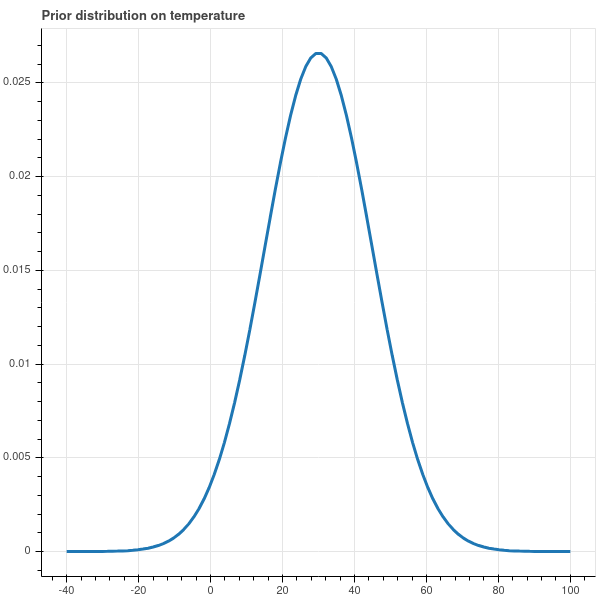
\includegraphics{../img/prior.png}
\caption{Prior Distribution on Temperature}\label{fig:tempprior}
}
\end{figure}

If we really have no opinion about the temperature other than its
between say, \(-20\) and \(100\) degrees, our prior distribution might
be uniform over that range, as in \cref{fig:uniformprior}.

\begin{figure}
\hypertarget{fig:uniformprior}{%
\centering
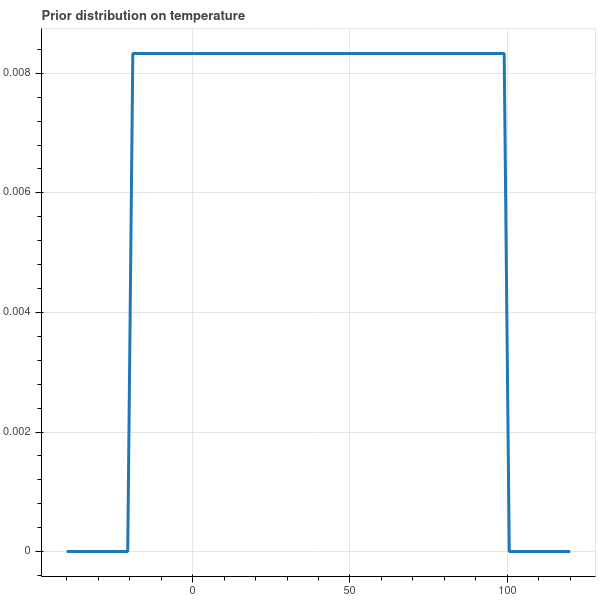
\includegraphics{../img/uniform.png}
\caption{Uniform Prior}\label{fig:uniformprior}
}
\end{figure}

The choice of a prior will guide the interpretation of our experiments
in ways that we will see shortly.

The next step in our experiment is the collection of data. Suppose we
let \(\mathbf{t}=(t_1,t_2,\ldots, t_n)\) be a random variable
representing \(n\) independent measurements of the temperature. We
consider the \emph{joint distribution} of the parameters \(t_*\) and
\(\sigma^2\) and the possible measurements \(\mathbf{t}\): \[
P(\mathbf{t},t_*,\sigma^2)=\left(\frac{1}{\sigma\sqrt{2\pi}}\right)^{n}e^{-\|\mathbf{t}-t_*\mathbf{e}\|^2/(2\sigma^2)}
\] where \(\mathbf{e}=(1,1,\ldots, 1)\).

The conditional probability \(P(t_{*},\sigma^2|\mathbf{t})\) is the
distribution of the values of \(t_*\) and \(\sigma^2\) \emph{given} a
value of the \(\mathbf{t}\). This is what we hope to learn by our
experiment -- namely, if we make a particular measurement, what does it
tell us about \(t_*\) and \(\sigma^2\)?

Now suppose that we actually make some measurements, and so we obtain a
specific set of values \(\mathbf{t}_0\) for \(\mathbf{t}\).

By Bayes Theorem, \[
P(t_{*},\sigma^2|\mathbf{t}=\mathbf{t}_0) = \frac{P(\mathbf{t}=\mathbf{t}_0|t_{*},\sigma^2)P(t_{*},\sigma^2)}{P(\mathbf{t}=\mathbf{t}_0)}
\] We interpret this as follows:

\begin{itemize}
\tightlist
\item
  the left hand side \(P(t_{*},\sigma^2|\mathbf{t}=\mathbf{t}_0)\) is
  called the \emph{posterior distribution} and is the distribution of
  \(t_{*}\) and \(\sigma^2\) obtained by \emph{updating our prior
  knowledge with the results of our experiment.}
\item
  The probability \(P(\mathbf{t}=\mathbf{t}_{0}|t_{*},\sigma^2)\) is the
  probability of obtaining the measurements we found for a particular
  value of the parameters \(t_{*}\) and \(\sigma^2\).
\item
  The probability \(P(t_{*},\sigma^2)\) is the \emph{prior distribution}
  on the parameters that reflects our initial impression of the
  distribution of these parameters.
\item
  The denominator \(P(\mathbf{t}=\mathbf{t}_{0})\) is the total
  probability of the results that we obtained, and is the integral over
  the distribution of the parameters weighted by their prior
  probability: \[
  P(\mathbf{t}=\mathbf{t}_{0})=\int_{t_{*},\sigma^2}P(\mathbf{t}=\mathbf{t}_{0}|t_{*},\sigma^2)P(t_{*},\sigma^2)
  \]
\end{itemize}

\hypertarget{bayesian-experiments-with-the-normal-distribution}{%
\subsubsection{Bayesian experiments with the normal
distribution}\label{bayesian-experiments-with-the-normal-distribution}}

To illustrate these Bayesian ideas, we'll consider the problem of
measuring the temperature, but for simplicity let's assume that we fix
the variance in our error measurements at \(1\) degree. Let's use the
prior distribution on the true temperature that I proposed in
\cref{fig:tempprior}, which is a normal distribution with variance
\(15\) ``shifted'' to be centered at \(30\): \[
P(t_*)=\left(\frac{1}{\sqrt{2\pi}}\right)e^{-(t_*-30)^2/30}.
\] The expected value \(E[t]\) -- the mean of the this distribution --
is \(30\).

Since the error in our measurements is normally distributed with
variance \(1\), we have \[
P(t-t_{*})=\left(\frac{1}{\sqrt{2\pi}}\right)e^{-(t-t_{*})^2/2}
\] or as a function of the absolute temperature, we have \[
P(t,t_{*}) = \left(\frac{1}{\sqrt{2\pi}}\right)e^{-(t-t_*)^2/2}.
\]

Now we make a bunch of measurements to obtain
\(\mathbf{t}_0=(t_1,\ldots, t_n)\). We have \[
P(\mathbf{t}=\mathbf{t}_0|t_{*}) = \left(\frac{1}{\sqrt{2\pi}}\right)^ne^{-(\mathbf{t}-t_*\mathbf{e})^2/2}.
\]

The total probability \(T=P(\mathbf{t}=\mathbf{t_0})\) is hard to
calculate, so let's table that for a while. The posterior probability is
\[
P(t_{*}|\mathbf{t}=\mathbf{t}_{0}) = \frac{1}{T} 
\left(\frac{1}{\sqrt{2\pi}}\right)^ne^{-\|\mathbf{t}-t_*\mathbf{e}\|^2/2}
\left(\frac{1}{\sqrt{2\pi}}\right)e^{-(t_*-30)^2/30}.
\]

Leaving aside the multiplicative constants for the moment, consider the
exponential \[
e^{-(\|\mathbf{t}-t_{*}\mathbf{e}\|^2/2+(t_{*}-30)^2)/30}.
\] Since \(\mathbf{t}\) is a vector of constants -- it is a vector of
our particular measurements -- the exponent \[
\|\mathbf{t}-t_{*}\mathbf{e}\|^2+(t_{*}-30)^2 = (t_{*}-30)^2/30+\sum_{i} (t_{i}-t_{*})^2/2
\] is a quadratic polynomial in \(t_{*}\) that simplifies: \[
(t_{*}-30)^2/30+\sum_{i} (t_{i}-t_{*})^2/2 = At_{*}^2+Bt_{*}+C.
\] Here \[
A=(\frac{1}{30}+\frac{n}{2}),
\] \[
B=-2-\sum_{i} t_{i}
\] \[
C=30+\frac{1}{2}\sum_{i} t_{i}^2.
\]

We can complete the square to write \[
At_{*}^2+Bt_{*}+C = (t_{*}-U)^2/2V +K
\] where \[
U=\frac{2+\sum_{i}t_{i}}{\frac{1}{15}+n}
\] and \[ 
V=\frac{1}{\frac{1}{15}+n}.
\] So up to constants that don't involve \(t_{*}\), the posterior
density is of the form \[
e^{(t_{*}-U)^2/2V}
\] and since it is a probability density, the constants must work out to
give total integral of \(1\). Therefore the posterior density is a
normal distribution centered at \(U\) and with variance \(V\). Here
\(U\) is called the \emph{posterior mean} and \(V\) the \emph{posterior
variance}.

To make this explicit, suppose \(n=5\) and we measured the following
temperatures: \[
40, 41,39, 37, 44
\] The mean of these observations is \(40.2\) and the variance is
\(5.4\).

A calculation shows that the posterior mean is \(40.1\) and the
posterior variance is \(0.2\). Comparing the prior with the posterior,
we obtain the plot in \cref{fig:comparison}. The posterior has a sharp
peak at \(40.1\) degrees. This value is just a bit smaller than the mean
of the observed temperatures which is \(40.2\) degrees. This difference
is caused by the prior -- our prior distribution said the temperature
was likely to be around \(30\) degrees, and so the prior pulls the
observed mean a bit towards the prior mean taking into account past
experience. Because the variance of the prior is large, it has a
relatively small influence on the posterior.

The general version of the calculation above is summarized in this
proposition.

\textbf{Proposition:} Suppose that our statistical model for an
experiment proposes that the measurements are normally distributed
around an (unknown) mean value of \(\mu\) with a (fixed) variance
\(\sigma^2\). Suppose further that our prior distribution on the unknown
mean \(\mu\) is normal with mean \(\mu_0\) and variance \(\tau^2\).
Suppose we make measurements \[
y_1,\ldots, y_n
\] with mean \(\overline{y}\). Then the posterior distribution of
\(\mu\) is again normal, with posterior variance \[
\tau'^2 = \frac{1}{\frac{1}{\tau^2}+\frac{n}{\sigma^2}}
\] and posterior mean \[
\mu' = \frac{\frac{\mu_0}{\tau^2}+\frac{n}{\sigma^2}\overline{y}}{\frac{1}{\frac{1}{\tau^2}+\frac{n}{\sigma^2}}}
\]

So the posterior mean is a sort of weighted average of the sample mean
and the prior mean; and as \(n\to\infty\), the posterior mean approaches
the sample mean -- in other words, as you get more data, the prior has
less and less influence on the results of the experiment.

\begin{figure}
\hypertarget{fig:comparison}{%
\centering
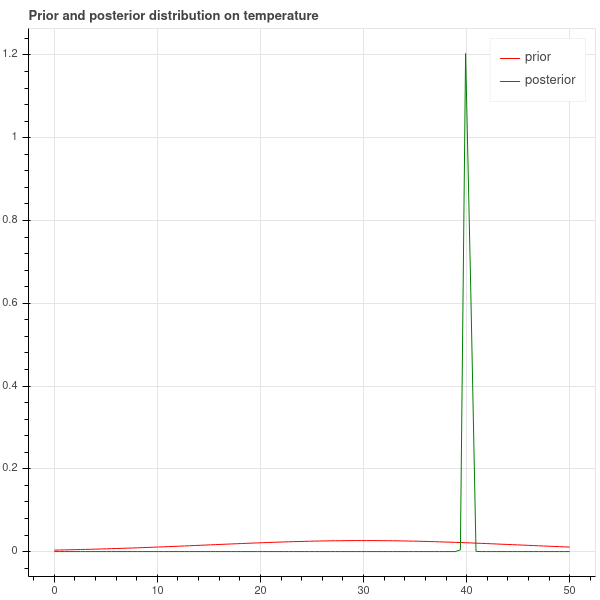
\includegraphics{../img/priorposterior.png}
\caption{Prior and Posterior}\label{fig:comparison}
}
\end{figure}

\hypertarget{bayesian-coin-flipping}{%
\subsubsection{Bayesian coin flipping}\label{bayesian-coin-flipping}}

For our final example in this fast overview of ideas from probability,
we consider the problem of deciding whether a coin is fair. Our
experiment consists of \(N\) flips of a coin with unknown probability
\(p\) of heads, so the data consists of the number \(h\) of heads out of
the \(N\) flips. To apply Bayesian reasoning, we need a prior
distribution on \(p\). Let's first assume that we have no reason to
prefer one value of \(p\) over another, and so we choose for our prior
the uniform distribution on \(p\) between \(0\) and \(1\).

We wish to analyze \(P(p|h)\), the probability distribution of \(p\)
given \(h\) heads out of \(N\) flips. Bayes Theorem gives us: \[
P(p|h) = \frac{P(h|p)P(p)}{P(h)}
\] where \[
P(h|p) = \binom{N}{h}p^{h}(1-p)^{N-h}
\] and \[
P(h)=\int_{p=0}^{1} P(h|p)P(p) dp = \binom{N}{h}\int_{p=0}^{1} p^{h}(1-p)^{N-h}dp
\] is a constant which insures that \[\int_{p}P(p|h)dp=1.\]

We see that the posterior distribution \(P(p|h)\) is proportional to the
polynomial function \[
P(p|h)\propto p^{h}(1-p)^{N-h}.
\] As in \cref{sec:mlcoin}, we see that this function peaks at \(h/N\).
This is called the maximum \emph{a posteriori estimate} for \(p\).

Another way to summarize the posterior distribution \(P(p|h)\) is to
look at the expected value of \(p\). This is called the \emph{posterior
mean} of \(p\). To compute it, we need to know the normalization
constant in the expression for \(P(p|h)\), and for that we can take
advantage of the properties of a special function \(B(a,b)\) called the
Beta-function: \[
B(a,b) = \int_{p=0}^{1} p^{a-1}(1-p)^{b-1} dp.
\]

\textbf{Proposition:} If \(a\) and \(b\) are integers, then
\(B(a,b)=\frac{a+b}{ab}\frac{1}{\binom{a+b}{a}}\).

\textbf{Proof:} Using integration by parts, one can show that \[
B(a,b)=\frac{a-1}{b}B(a-1,b+1)
\] and a simple calculation shows that \[
B(1,b) = \frac{1}{b}.
\] Let \[
H(a,b)=\frac{a+b}{ab}\frac{1}{\binom{a+b}{a}} = \frac{(a-1)!(b-1)!}{(a+b-1)!}
\] Then it's easy to check that \(H\) satsifies the same recurrences as
\(B(a,b)\), and that \(H(1,b)=1/b\). So the two functions agree by
induction.

Using this Proposition, we see that \[
P(p|h) = \frac{p^{h}(1-p)^{N-h}}{B(h+1,N-h+1)}
\] and \[
E[p] = \frac{\int_{p=0}^{1} p^{h+1}(1-p)^{N-h}dp}{B(h+1,N-h+1)}=\frac{B(h+2,N-h+1)}{B(h+1,N-h+1)}.
\] Sorting through this using the formula for \(B(a,b)\) we obtain \[
E[p]=\frac{h+1}{N+2}.
\]

So if we obtained \(55\) heads out of \(100\) flips, the maximum a
posteriori estimate for \(p\) is \(.55\), while the posterior mean is
\(56/102=.549\) -- just a bit less.

Now suppose that we had some reason to believe that our coin was fair.
Then we can choose a prior probability distribution that expresses this.
For example, we can choose \[
P(p) = \frac{1}{B(5,5)}p^{4}(1-p)^{4}.
\] Here we use the Beta function to guarantee that
\(\int_{0}^{1}P(p)dp=1\). We show this prior distribution in
\cref{fig:betaprior}.

\begin{figure}
\hypertarget{fig:betaprior}{%
\centering
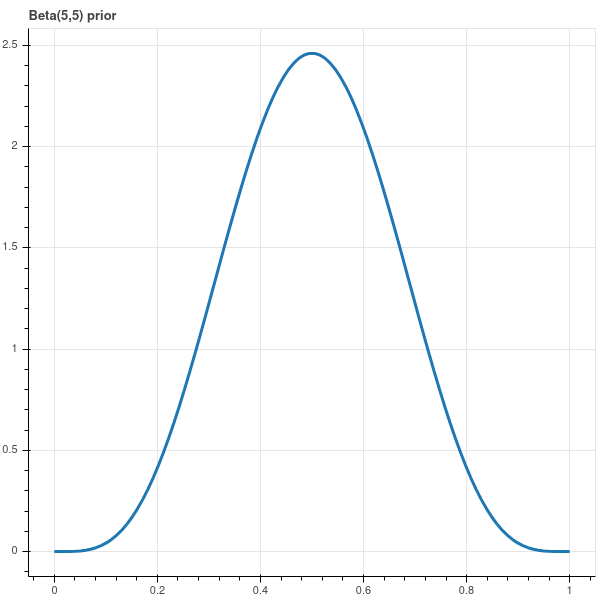
\includegraphics{../img/betaprior.png}
\caption{Beta(5,5) Prior}\label{fig:betaprior}
}
\end{figure}

If we redo our Bayes theorem calculation, we find that our posterior
distribution is \[
P(p|h) \propto p^{h+4}(1-p)^{N-h+4}
\] and relying again on the Beta function for normalization we have \[
P(p|h) = \frac{1}{B(h+5,N-h+5)}p^{h+4}(1-p)^{N-h+4}
\] Here the maximum a posterior estimate for \(p\) is \(h+4/N+8\) while
our posterior mean is \[
\frac{B(h+6,N-h+5)}{B(h+5,N-h+5)} = \frac{h+5}{N+10}.
\]

In the situation of \(55\) heads out of \(100\), the maximum a
posteriori estimate is \(.546\) and the posterior mean is \(.545\).
These numbers have been pulled just a bit towards \(.5\) because our
prior knowledge makes us a little bit biased towards \(p=.5\).

\hypertarget{bibliography}{%
\section*{References}\label{bibliography}}
\addcontentsline{toc}{section}{References}

\hypertarget{refs}{}
\begin{CSLReferences}{0}{0}
\leavevmode\hypertarget{ref-Bertsekas}{}%
\CSLLeftMargin{{[}1{]} }
\CSLRightInline{\textsc{Bertsekas}, D. P. and \textsc{Tsitsiklis}, J. N.
(2008). \emph{Introduction to probability}. Athena Scientific.}

\end{CSLReferences}

\end{document}
